\documentclass{article}
\usepackage{iclr2026_conference,times}
\usepackage[hidelinks,pdfstartview={}]{hyperref}
\usepackage{url}
\usepackage{booktabs}
\usepackage{amsmath,amssymb}
\usepackage{graphicx}
\usepackage{xcolor}
\usepackage{microtype}
\usepackage{enumitem}
\usepackage{multirow}
\usepackage{makecell}
\usepackage[capitalise,noabbrev]{cleveref}
\setlist{itemsep=2pt,topsep=3pt}

\title{EPACT: Vision--Language Agents Can Use\\Evidence They Cannot Acquire}

\usepackage[T1]{fontenc}
\iclrfinalcopy
\author{Yixuan Yang\\Independent researcher}
\begin{document}
\maketitle
\lhead{Preprint}

\begin{abstract}
Embodied question answering couples two abilities that benchmarks usually score together: acquiring an informative observation and using it. EPACT separates them with answer-flipped world pairs in ProcTHOR: both members share the house, question and starting pose, but a hidden object's presence or state flips the answer, so a constant answer earns no credit. Task families make the evidence hard to reach, and each pair is evaluated from the start view, from a supplied evidence view, under autonomous interaction and after a replayed acquisition prefix. Across Qwen3-VL-2B, 8B and 30B-A3B, a supplied evidence image yields 44--57 of 72 correct pairs and autonomous interaction 7--8, with no corresponding autonomous gain across these three model sizes. A replayed acquisition prefix recovers only 16--26 pairs: the 8B policy fails 20 of the 44 pairs whose handoff view it can answer, usually by repeating an action whose result it has already seen. Trajectory fine-tuning on 87 pairs raises the 8B model to 34--42 pairs across three seeds but transfers inspection routines more consistently than the choice of intervention: without lighting demonstrations, models improve on dark rooms without ever turning on a light, and without container demonstrations only one of three seeds opens containers. A reason-first prompt elicits container opening from both base and fine-tuned models, and source-family RL shows a small advantage over step-matched SFT, though a reliable transfer benefit remains unconfirmed. After acquisition, reading remains an obstacle: policies that open the container in nearly every egg episode still solve at most 4 of 19 egg pairs. EPACT makes the acquisition gap measurable and shows where training does and does not close it.
\end{abstract}

\section{Introduction}

A vision--language model can answer correctly when shown the inside of a refrigerator, yet fail to open the refrigerator when asked what it contains. Embodied question answering \citep{das2018embodied,gordon2018iqa} and its foundation-model successors \citep{majumdar2024openeqa} evaluate a chain of decisions: making an informative observation available, interpreting it, and committing to an answer once the evidence suffices. A single success rate cannot tell which link failed, and therefore cannot tell what training should fix. Recent evidence audits likewise show why answer accuracy alone does not establish that an agent acquired supporting observations \citep{garg2026answering}.

EPACT is a diagnostic benchmark built to separate these links. Its unit is an \emph{answer-flipped pair}: two episodes that share the house, the question and the starting configuration, but differ in the presence or state of a hidden object, which flips the answer (\cref{fig:pair}): an egg is in the refrigerator in one world and absent in the other. Task families vary what makes that evidence hard to reach: a closed container, a dark room, distance. A policy that always answers ``yes'' or always answers ``no'' scores zero pairs, even though it is right on half of the episodes. Each pair is evaluated under five conditions that supply different amounts of help: the start view alone, a supplied evidence view, autonomous interaction, a replayed acquisition prefix followed by autonomous completion, and the exact view reached by that prefix.

The decomposition exposes a large gap (\cref{fig:teaser}). Supplied with one evidence image, frozen Qwen3-VL models \citep{bai2025qwen3vl} answer 44--57 of 72 development pairs correctly; acting on their own, they solve 7--8. The gap does not shrink from 2B to 30B-A3B parameters. Even when a replayed prefix delivers the agent to an answerable view, the 8B policy completes only about half of the pairs it could answer from that view, often by repeating an observation action until the decision limit.

We organize the study around six questions. \textbf{Q1:} do frozen models use evidence they cannot acquire? The gap above answers yes (\cref{sec:gap}). \textbf{Q2:} can demonstrations close the gap on the families they cover? Trajectory supervision on 87 training pairs lifts the 8B model from 8 to 34--42 pairs across three seeds. \textbf{Q3:} what transfers to families withheld from the demonstrations? Inspection routines (approach, aim, commit) carry over to dark rooms without the model ever turning on a light, while opening a container is not reliably selected when it is absent from the demonstrations. Transfer thus remains unreliable at the choice of intervention, which leaves two ways to change that choice. \textbf{Q4:} is the missing action lost, or can a different response context elicit it? A reason-first prompt elicits opening from base and fine-tuned models alike. \textbf{Q5:} can rewards on the outcomes of self-selected actions improve transferable intervention selection? A source-family RL continuation shows a small advantage over step-matched SFT, suggesting a possible transfer benefit. \textbf{Q6:} what still fails once the evidence has been acquired? On the container target, rendered eggs expose a further obstacle after acquisition: policies open the queried container in nearly every egg episode yet solve at most 4 of the 19 egg pairs, and an environment-specific class note repairs most egg confusions in a small witness subset, at a cost on other objects.

\paragraph{Contributions.}
\begin{itemize}
\item \textbf{A paired benchmark that separates evidence use from evidence acquisition.} Answer-flipped pairs remove constant-answer credit, and five evaluation conditions isolate answerability, acquisition and completion on the same items (\cref{sec:bench}).
\item \textbf{A measured acquisition gap.} Frozen VLMs solve 5.5--8$\times$ more pairs from supplied evidence than through autonomous interaction, with no corresponding autonomous gain across the three tested model sizes, and fail to complete many tasks whose evidence they have already reached (\cref{sec:gap}).
\item \textbf{A map of what training changes.} Trajectory SFT closes much of the in-distribution gap; transfer, elicitation and RL experiments show that it improves inspection procedures without reliably transferring the selection of specific epistemic actions (Q2--Q5, \cref{sec:training}).
\item \textbf{A diagnosis of failures after acquisition.} Splitting the container target by question object, with recorded witness images and a class-note probe whose collateral errors are reported alongside its gains, locates the remaining egg errors in reading rather than opening (Q6, \cref{sec:localized}).
\end{itemize}

\begin{figure}[t]
\centering
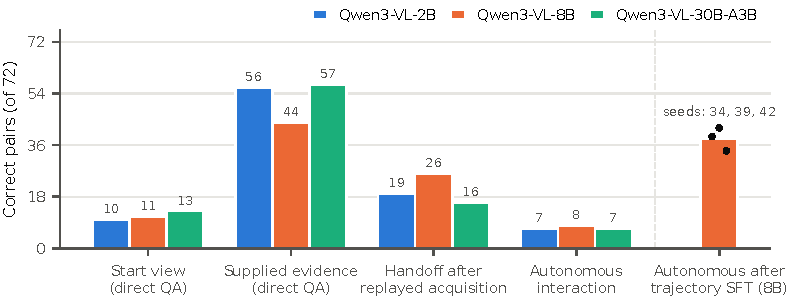
\includegraphics[width=\linewidth]{figures/epact_fig_teaser.pdf}
\caption{\textbf{Models can use evidence they cannot acquire.} Correct pairs out of 72 development pairs for three frozen Qwen3-VL models under four evaluation conditions, and for the 8B model after trajectory SFT (bar: mean of three seeds; dots: seeds). A pair counts only if both answer-flipped members are correct.}
\label{fig:teaser}
\end{figure}

\section{Related work}

\paragraph{Embodied question answering.} EQA formulated question answering as a task in which an agent must move through a 3D environment to collect observations \citep{das2018embodied}; IQA extended it to interaction with objects, including opening containers \citep{gordon2018iqa}. OpenEQA evaluates foundation models both with an episodic memory of the scene and in an active exploration setting \citep{majumdar2024openeqa}, and \citet{ren2024explore} calibrate exploration so that an agent stops once it is confident. EPACT keeps the question format but changes the unit of evaluation: the same answer-flipped pairs are scored with supplied evidence, autonomously and after assisted acquisition, and the hidden states are chosen so that an action (opening, switching on a light, approaching) is what makes the answer visible.

\paragraph{Evidence acquisition and diagnostic evaluation.} ESI-Bench evaluates active spatial reasoning through viewpoint changes and physical interaction, and identifies poor action selection as a source of inadequate observations \citep{hong2026esibench}. \citet{garg2026answering} compare evidence-access conditions on fixed multi-room questions and audit shortcuts that allow answers without supporting observations. EviSeek makes the evidence required by a question an explicit target for acquisition and memory selection \citep{li2026eviseek}. EPACT centers evaluation on answer-flipped world pairs, so a constant answer receives no paired credit, and combines supplied views, autonomous interaction and acquisition handoffs on those pairs. Its training and held-out-family probes then ask whether an observed acquisition gap can be reduced and which inspection behaviors transfer.

\paragraph{Benchmarks for VLM and LLM agents.} ALFRED \citep{shridhar2020alfred}, the Embodied Agent Interface \citep{li2024embodied} and EmbodiedBench \citep{yang2025embodiedbench} evaluate language and vision--language models as embodied agents across many tasks and report where they fail. EPACT is narrower and diagnostic: it holds the question fixed and varies the route to evidence. Its contrasts also differ in prompt and output format, so they diagnose where performance changes rather than isolating a single mechanism.

\paragraph{Active and interactive perception.} The idea that perception should control the sensor rather than passively receive data goes back to active perception \citep{bajcsy1988active}; interactive perception extends it to physical actions that reveal information \citep{bohg2017interactive}. EPACT measures whether modern VLM policies exhibit this behavior at the level of high-level epistemic actions.

\paragraph{Training interactive policies.} Our trajectory training is behavior cloning on demonstrated states, whose train--deployment mismatch is well known \citep{ross2011reduction}; our RL continuation uses a group-relative policy gradient in the style of GRPO \citep{shao2024deepseekmath}, and our reason-first prompt asks for reasoning before the action, as in ReAct \citep{yao2023react}. We use AI2-THOR and ProcTHOR \citep{kolve2017ai2thor,deitke2022procthor} and adapt models with LoRA \citep{hu2022lora}.

\section{The EPACT benchmark}
\label{sec:bench}

\subsection{Interaction interface}
A task consists of a scene, a starting agent pose, a question and a hidden answer derived from the scene configuration. At each decision step the policy receives the current RGB image, the question, public action instructions and a bounded text history of recent actions and execution feedback, and emits one structured action, for example \texttt{\{"action":"Open","args":\{"target":"query\_location"\}\}}. The environment executes it and renders the next observation; an \texttt{Answer} action ends the episode. The principal actions are \texttt{GoTo} (move to an interaction pose with a chosen distance, side or stance), \texttt{LookAt} (adjust the view), \texttt{Open} and \texttt{Toggle}. The benchmark therefore concentrates on choosing and sequencing information-acquisition actions; it does not evaluate collision-free motor control or continuous manipulation.

Public aliases name task roles: \texttt{query\_location} is the location named in the question, \texttt{query\_object} an explicitly queried state-bearing entity, and \texttt{room\_light} an available lighting control. Presence questions do not allow direct addressing of the object whose existence is being tested, so a lookup cannot substitute for visual inspection. A successful execution message means only that the operation ran, not that the resulting image suffices to answer.

\subsection{Answer-flipped pairs}
For a presence question, the paired worlds share the house, question and initial agent configuration, but the queried object is present in one world and absent in the other; state questions vary the relevant state in the same way (\cref{fig:pair}). The two episodes are evaluated independently. With $c(i,0)$ and $c(i,1)$ the correctness indicators of the members of pair $i$,
\begin{equation}
S_{\text{pair}} = \frac{1}{N}\sum_{i=1}^{N} c(i,0)\,c(i,1).
\end{equation}
A policy that always returns the same answer scores zero pairs while obtaining 50\% member accuracy. Pair success does not by itself show that a particular action was necessary, so we also inspect action execution and termination.

\begin{figure}[t]
\centering
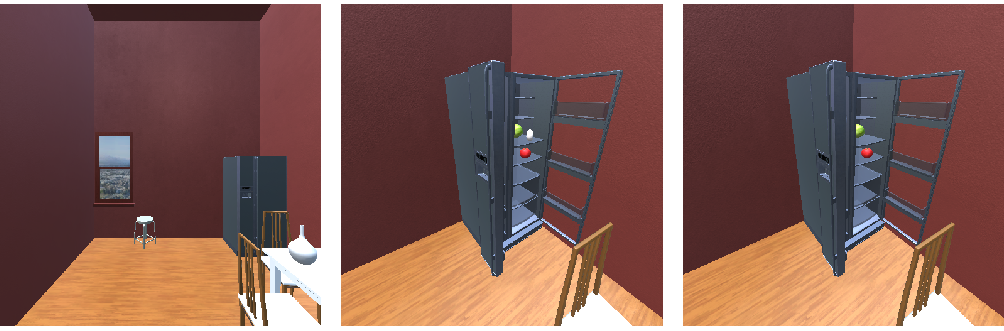
\includegraphics[width=0.86\linewidth]{figures/epact_fig_pair.pdf}
\caption{\textbf{An answer-flipped container pair.} The question asks whether an egg is in the refrigerator. Left: the shared initial observation. Middle and right: inspection views of the positive and negative worlds; the egg is present only in the middle image.}
\label{fig:pair}
\end{figure}

\subsection{Task families}
Task families vary how evidence becomes available (\cref{tab:families} in \cref{app:details}). Container tasks (C) place the relevant contents behind a closed receptacle. Distance and viewpoint tasks (D) require a more informative view. Lighting tasks (L) place the scene in a dark room with an available light switch, implemented as a conditional RGB attenuation of about 0.04 that \texttt{Toggle} removes (\cref{fig:light}); residual image structure can sometimes support an answer without toggling, so membership in L does not guarantee that toggling is necessary. Combined families (C+D, L+D, D+door) test conditions together, neutral tasks (N) are readable from the start, and state tasks (STATE$|$D) ask about an object's state under a distance condition. The training set contains 174 episodes from 52 ProcTHOR training houses and the development set 144 episodes from 37 validation houses; the two are house-disjoint.


\subsection{Five evaluation conditions}
Each pair is evaluated under five conditions (\cref{tab:conditions}). A \emph{witness} is a selected observation intended to make the answer visually accessible; it is an empirical reference rather than an upper bound, because the same model can behave differently under a direct QA prompt and an interactive policy prompt. \emph{Handoff} replays a recorded public-action prefix and then returns control to the model, which receives the resulting observation and history but is not told that the evidence suffices. Because the intervention supplies both a state and a history, its effect should not be read as a pure navigation improvement.

\begin{table}[t]
\centering
\caption{Evaluation conditions. Direct QA answers without controlling the environment.}
\label{tab:conditions}
\small
\begin{tabular}{p{2.5cm}p{5.3cm}p{4.9cm}}
\toprule
Condition & Input or intervention & What it measures \\
\midrule
Start QA & Initial image, direct QA prompt & Answerability before interaction \\
Witness QA & Selected evidence image, direct QA prompt & Answerability with supplied evidence \\
Autonomous & Original start, action policy & Acquisition and completion together \\
Handoff & Replayed acquisition prefix, then the policy & Completion after assisted acquisition \\
Fresh handoff QA & The newly rendered handoff image, direct QA & Readability of the handoff view \\
\bottomrule
\end{tabular}
\end{table}

\subsection{Scoring rules}
Interactive episodes allow at most 14 decisions, including the \texttt{Answer} and any handoff prefix. The model sees the current $512\times512$ image and the last six text action--feedback entries; earlier images are not retained, and no simulator metadata or ground-truth answer is passed to it. Decisions use a fresh model call with greedy decoding and at most 96 generated tokens (48 for direct QA). An episode that reaches the decision limit or otherwise ends without a valid model \texttt{Answer} is unsuccessful; a fallback answer recorded by the harness is not credited. We distinguish emitting an \texttt{Open} action from successfully opening the queried container, which requires a successful native operation on the intended receptacle; this separates missing action selection, failed execution and incorrect completion.

\section{The use--acquisition gap in frozen models}
\label{sec:gap}

\begin{table}[t]
\centering
\caption{\textbf{Supplied evidence is used; acquisition fails.} Correct pairs out of 72 for frozen instruction-tuned models, with 95\% Wilson intervals (in \%). Witness and fresh-handoff images are rendered in separate runs, so their scores can differ.}
\label{tab:frozen}
\small
\begin{tabular}{lccccc}
\toprule
Frozen model & Start QA & Witness QA & Autonomous & Handoff & Fresh handoff QA \\
\midrule
Qwen3-VL-2B & 10 \,{\scriptsize[8, 24]} & 56 \,{\scriptsize[67, 86]} & 7 \,{\scriptsize[5, 19]} & 19 \,{\scriptsize[18, 38]} & 57 \,{\scriptsize[68, 87]} \\
Qwen3-VL-8B & 11 \,{\scriptsize[9, 25]} & 44 \,{\scriptsize[50, 72]} & 8 \,{\scriptsize[6, 20]} & 26 \,{\scriptsize[26, 48]} & 44 \,{\scriptsize[50, 72]} \\
Qwen3-VL-30B-A3B & 13 \,{\scriptsize[11, 28]} & 57 \,{\scriptsize[68, 87]} & 7 \,{\scriptsize[5, 19]} & 16 \,{\scriptsize[14, 33]} & 58 \,{\scriptsize[70, 88]} \\
\bottomrule
\end{tabular}
\end{table}

We first ask whether frozen models can use evidence that they fail to acquire (Q1). \Cref{tab:frozen} and \cref{fig:teaser} show the central result. Across three models, supplying an evidence image yields 44--57 correct pairs, whereas autonomous interaction yields 7--8; the intervals do not overlap. Larger models do not solve the interaction problem under this interface. Start-view QA (10--13 pairs) confirms that the tasks are rarely answerable without acquiring evidence. Handoff raises success to 16--26 pairs, so an acquisition prefix helps, but the policy still falls well short of direct QA on the very images it reaches.

\subsection{Readable evidence can coexist with failed completion}
For the frozen 8B model, fresh handoff QA answers both members correctly on 44 pairs; on those same 44 pairs the handoff policy solves 24 (its overall handoff score of 26 includes two pairs outside this subset). The remaining 20 pairs contain 22 failed episodes: 21 repeat observation actions until the decision limit, and one produces an incorrect answer.



\Cref{fig:handoff} in \cref{app:details} shows one case. In a distance task asking whether a tissue box is on a bathroom side table, direct QA succeeds on both handoff images; in the positive episode the policy instead emits the same \texttt{LookAt} twelve times and never answers. In another case, about a book on a dining table, the policy repeats \texttt{LookAt} three times and then answers ``no'' in both worlds, although direct QA answers both correctly from the unchanged images. Repetition can become self-maintaining in this interface: once the six-entry history contains only identical successful \texttt{LookAt} operations, the image and rendered history can repeat exactly and greedy decoding receives the same input again. Successful tool execution carries no signal that the action added no information. These cases establish an observable distinction between image answerability and policy completion; they do not reveal an internal answer that the policy has already computed, since direct QA and action generation use different contexts.

\section{Can training close the gap?}
\label{sec:training}

\subsection{Demonstrations and adaptation}
A programmatic demonstrator uses scene metadata and task conditions to construct candidate inspection routes: it identifies the relevant receptacle, inspects object states, chooses interaction poses and tests views. Candidate observations are filtered by visible target pixels and coverage of the relevant region, with additional visual review; the training pool contains 46 automatically screened pairs and 41 pairs selected through assistant-aided visual review. Positive and negative answers require different evidence: seeing the queried object supports ``yes'', while an absence judgment requires sufficient coverage of where it would appear. Scene truth supplies the answer label; observation selection supplies useful evidence for it.

Selected routes are replayed through the public interface. Before each action we record the current image and exact policy context and pair it with the next demonstrated action; at the endpoint we add an \texttt{Answer} target. Action supervision is kept only when both members of a pair share the same successful action prefix, so that answer-specific route differences cannot act as a label cue (one pair with asymmetric prefixes contributes answer rows only). The full dataset has 724 state--action examples: 304 \texttt{GoTo}, 168 \texttt{LookAt}, 36 \texttt{Open}, 42 \texttt{Toggle} and 174 \texttt{Answer}. We minimize next-token cross-entropy on the demonstrated action string; there is no separate information-gain reward or sufficiency classifier.

We adapt Qwen3-VL-8B-Instruct with rank-16 LoRA on the language attention projections for one epoch, keeping the base model and vision encoder frozen; each of three seeds starts from the base model (hyperparameters in \cref{app:details}). Answer-only training uses the terminal examples alone, so it holds final-answer supervision fixed while trajectory training adds rows and updates; we treat the comparison as one between training packages rather than a compute-matched isolation of action labels.

\subsection{Q2: trajectory SFT closes much of the in-distribution gap}
Q2 asks whether demonstrations close the gap on the families they cover. Full trajectory SFT raises autonomous performance in every seed, to 39, 42 and 34 correct pairs (mean 38.3, against 8 for the frozen model). Distance and lighting families improve most (\cref{tab:families_sft} in \cref{app:details}). Container completion and the three-pair door subset remain difficult: the policies successfully open the queried container in 40, 38 and 35 of 40 container episodes, yet solve only 6, 6 and 7 of the 20 C and C+D pairs. Executing the enabling action is an intermediate achievement, not a guarantee of success; identifying the causes of these residual errors requires direct QA on the actual rollout observations.


\subsection{Q3: inspection routines transfer more reliably than interventions}
\label{sec:transfer}
Q3 asks what a policy carries to a family whose demonstrations it never saw. Two held-out-family experiments remove a demonstration family from training and test on it zero-shot. These hold out demonstrations, not concepts: the tools and ideas may still be known from pretraining.

\paragraph{Lighting without light switches.} The lighting-transfer experiment trains on C, D and C+D only: 43 pairs (27 original training pairs plus 16 from the development source pool, chosen from houses disjoint from all evaluation houses), 39 houses and 458 rows (372 action targets, 86 answers), with no \texttt{Toggle} demonstration. Evaluation uses L, L+D and N, ten pairs each across 21 houses; these adapters are evaluated only on this transfer set and are not comparable to full-set scores.

\begin{table}[t]
\centering
\caption{\textbf{Transfer to dark rooms happens without turning on the light.} Correct pairs on families excluded from training (C/D/C+D training only).}
\label{tab:light}
\begin{tabular}{lrrrr}
\toprule
Training condition & L /10 & L+D /10 & N /10 & Total /30 \\
\midrule
Frozen 8B & 1 & 0 & 3 & 4 \\
Trajectory SFT, seeds 1/2/3 & 5 / 3 / 6 & 5 / 3 / 5 & 7 / 7 / 5 & 17 / 13 / 16 \\
Answer-only SFT, seeds 1/2/3 & 3 / 3 / 3 & 0 / 0 / 0 & 7 / 7 / 8 & 10 / 10 / 11 \\
\bottomrule
\end{tabular}
\end{table}

On L and L+D together, trajectory models solve 10, 6 and 11 of 20 pairs, compared with 3 for every answer-only seed and 1 for the frozen model (\cref{tab:light}). Yet none of the trajectory models ever attempts \texttt{Toggle}; their successes come from approach-and-look routines that exploit improved views and residual visibility. All 180 trajectory-model episodes begin with an action and 179 end with an autonomous answer, whereas all 180 answer-only episodes answer immediately. Acting in every neutral episode also indicates a learned preference for inspection rather than a selective decision to act only when evidence is insufficient. Useful interactive behavior transfers; a lighting-specific intervention is not acquired.

\paragraph{Containers without opening demonstrations.} The container-transfer experiment removes all C, C+D and D+door training pairs. The remaining 69 pairs span N, D, L, L+D and STATE$|$D across 41 training houses (510 rows: 194 \texttt{GoTo}, 136 \texttt{LookAt}, 42 \texttt{Toggle}, 138 \texttt{Answer}). \texttt{Open} appears in neither targets nor histories, while the tool description and permission to invoke it remain. Evaluation uses the 20 C and C+D development pairs across 17 houses.

\begin{table}[t]
\centering
\caption{\textbf{Opening without demonstrations is inconsistent across seeds.} Transfer to container tasks after excluding all opening demonstrations. Full-data rows are contextual references with a different training scope and size.}
\label{tab:noopen}
\begin{tabular}{lcc}
\toprule
Condition & Container pairs /20 & Successful target-opening episodes /40 \\
\midrule
Frozen 8B & 1 & 4 \\
No-Open SFT, seeds 1/2/3 & 0 / 0 / 2 & 0 / 0 / 19 \\
Full SFT, seeds 1/2/3 & 6 / 6 / 7 & 40 / 38 / 35 \\
\bottomrule
\end{tabular}
\end{table}

The first two no-Open seeds use the exact sequence \texttt{GoTo}, \texttt{LookAt}, \texttt{Answer(no)} in all 40 episodes (\cref{tab:noopen}). They complete normally but never open the container, and their 50\% member accuracy becomes zero pair success, exposing a uniform absence response. The third seed opens the queried container in 19 episodes and solves two pairs, while 15 episodes reach the decision limit and seven of its 19 opening episodes still end with an incorrect answer. Opening is possible without demonstrations but does not transfer reliably. Together with the lighting result, this separates transferring a general observation routine from reliably selecting a particular tool to overcome a particular information barrier.

\paragraph{From transfer to action selection.} Both experiments leave the same gap: in a new family the trained policies approach, aim and answer, but they do not reliably select the intervention associated with the family's information barrier. What could fix this depends on why. If opening is no longer available to the fine-tuned weights, a different prompt cannot recover it; if it is available but not selected, a different response context might elicit it (Q4, \cref{sec:reason}), and rewards on the outcomes of actions the policy selects itself might improve the selection that demonstrations failed to transfer (Q5, \cref{sec:rl}).

\subsection{Q4: reasoning elicits a preserved procedure}
\label{sec:reason}
The no-Open failure does not by itself show that SFT erased the pretrained opening behavior. A probe on 20 training-house container pairs (40 episodes, sampling at temperature 1) replaces the immediate-JSON instruction with a reason-first protocol: the model reasons, the output allowance rises from 96 to 256 tokens, and the final balanced action JSON is parsed. These changes form one bundled elicitation protocol.



Under this protocol the base model opens the queried container in 22 of the 40 episodes, answers 19 correctly and ends 11 without a valid answer; no-Open SFT seed 1 opens in 27, answers 22 correctly and ends 5 without a valid answer. Reason-first thus brings the base and fine-tuned models into a similar behavioral range, whereas under sampled immediate-action evaluation the same SFT model opens in only 1 of the 40 episodes (the historical base immediate-action reference, 4 of 40, is not a matched sampled cell). The same protocol, run greedily, defines the \emph{container target} used for the rest of this section: 55 pairs, 32 human-reviewed (segment A) and 23 machine-validated (segment B), which we also split by question object into 19 egg pairs and 36 other pairs (\cref{tab:target}). On this target the base model opens the queried container in 52 of 110 episodes and the three no-Open SFT seeds in 56, 56 and 55. Opening therefore remains available to the fine-tuned weights and can be elicited. This does not rule out damage under the immediate-action protocol, where the same SFT model opens in only 1 of 40 sampled episodes.

\begin{table}[t]
\centering
\caption{\textbf{On the container target, opening is common while egg pairs are rarely solved.} Greedy reason-first evaluation on 55 container pairs; these rows should not be compared with the earlier action-only tables. Egg and Other split the pairs by question object. Opened: episodes that successfully open the queried container. Light-call episodes: episodes with at least one \texttt{GoTo} or \texttt{Toggle} targeting \texttt{room\_light} (issued calls, not successful interventions; not computed for the answer-only model). Rows below the rule are introduced in \cref{sec:rl}.}
\label{tab:target}
\small
\setlength{\tabcolsep}{4.5pt}
\begin{tabular}{lccccccc}
\toprule
Policy & \makecell{Pairs\\/55} & \makecell{Seg.\ A\\/32} & \makecell{Seg.\ B\\/23} & \makecell{Egg\\/19} & \makecell{Other\\/36} & \makecell{Opened\\/110} & \makecell{Light-call\\episodes /110} \\
\midrule
Base & 11 & 8 & 3 & 2 & 9 & 52 & 0 \\
No-Open SFT seed 1 (A0) & 19 & 10 & 9 & 2 & 17 & 56 & 1 \\
No-Open SFT seed 2 & 10 & 8 & 2 & 2 & 8 & 56 & 19 \\
No-Open SFT seed 3 & 14 & 8 & 6 & 1 & 13 & 55 & 9 \\
Answer-only SFT & 1 & 1 & 0 & 0 & 1 & 10 & -- \\
\midrule
A1: source RL & 17 & 11 & 6 & 3 & 14 & 61 & 0 \\
A2: step-matched source SFT & 14 & 10 & 4 & 3 & 11 & 61 & 0 \\
P: container-family RL & 21 & 12 & 9 & 4 & 17 & 56 & 0 \\
\bottomrule
\end{tabular}
\end{table}

Pair success varies more than opening: 11 of 55 for the base model against 19, 10 and 14 for the SFT seeds; the two replication seeds average 12. The seeds also differ in which routine they call. Seed 1 issues a \texttt{GoTo} or \texttt{Toggle} targeting \texttt{room\_light} in 1 of 110 container episodes, seed 3 in 9 and seed 2 in 19 (1, 17 and 37 such calls in total), and their scores on non-egg pairs fall in the same order (17, 13 and 8 of 36), while egg pairs stay at 1--2 of 19. Three seeds give a descriptive association rather than an isolated effect, but the pattern fits one reading: fine-tuning installs procedures whose selection the response context controls, here a lighting routine of the kind demonstrated for dark rooms, called in container tasks whose barrier is a closed receptacle. A diagnostic in the opposite direction trains a fresh base model on the 138 answer rows alone for 64 updates: it solves 1 of 55 pairs, answers ``no'' in 101 of 110 episodes and opens the queried container in only ten, consistent with premature commitment when answers are supervised without the preceding inspection. The SFT update is small (rank-16 attention LoRA, about 15.3 million parameters, roughly one epoch of action-JSON supervision), which may help explain why opening survives, although rank, modules, dose and target format were not manipulated independently.

\subsection{Q5: source-family RL shows a tentative transfer advantage}
\label{sec:rl}
The transfer results motivate a direct test of Q5: if a policy is rewarded for the outcomes of actions it selects itself on source families, does it select interventions better on held-out container tasks? A0 is the first no-Open SFT seed; A1 continues A0 with source-family RL; A2 continues it with additional source SFT matched to A1's number of optimizer updates; P is a container-family RL reference, not a compute-matched transfer control. All are evaluated on the container target with the greedy reason-first protocol.

The source pool contains 115 pairs (23 in each of D, L, L+D, N and STATE$|$D). Each update draws five twin pairs with four sampled rollouts per member, giving eight rollouts per twin group, with binary reward for autonomous correctness and no opening bonus or step penalty. We use a group-relative advantage $A_e = r_e - \bar r_g$ and a policy gradient over all sampled assistant tokens, including reasoning and action JSON, with a KL penalty to the starting policy (details in \cref{app:rl}). A1 executes 120 updates over 600 twin groups (4,800 rollout episodes); A2 matches the 120 updates.

A1 solves 17 of 55 pairs against 14 for A2, a three-pair advantage, one of them on segment A; both policies open in 61 episodes (\cref{tab:target}). The direction suggests a possible transfer benefit from source-family RL, but this single-initialization comparison does not establish that the improvement is reliable. In the 4,800 A1 rollouts there are six non-container \texttt{Open} actions and no container opening, which constrains what source rewards could have reinforced.

Neither continuation keeps A0's score. A1 and A2 fall below A0 on non-egg pairs (14 and 11 of 36, against 17), and the loss lies mostly in segment B (A0 9, A1 6, A2 4 of its 21 non-egg pairs), where A0 solves its pairs without attempting \texttt{Open} in any episode. Neither continuation calls \texttt{room\_light} in any of its 110 episodes, so the lighting association of \cref{sec:reason} does not explain this decline, and the recorded diagnostics do not identify its cause. P, trained with container rewards, ties A0 on non-egg pairs (17 of 36); its two-pair lead lies entirely in egg pairs (4 against 2 of 19).

\subsection{Q6: after the container opens, eggs remain hard to read}
\label{sec:localized}
Q6 asks what fails once the evidence has been acquired. The container target is concentrated: segment A contains 27 refrigerator pairs, and egg questions make up 17 of its 32 pairs and 2 of segment B's 23 (19 of 55). Every policy except the answer-only model opens the queried container in at least 36 of the 38 egg episodes, yet none solves more than 4 of the 19 egg pairs (\cref{tab:target}). On these items the bottleneck lies after acquisition. Saved images and traces show errors in both directions, rendered eggs missed in an opened refrigerator and ovoid distractors reported as eggs (\cref{fig:egg}), as well as failures to use a newly available view.

\begin{figure}[t]
\centering
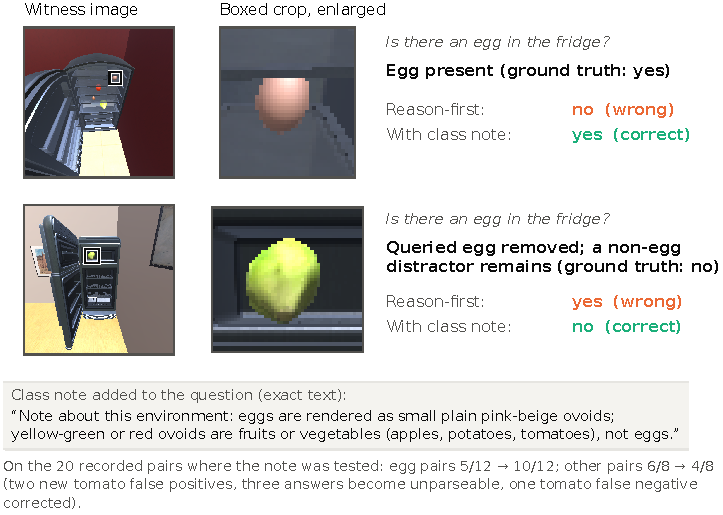
\includegraphics[width=\linewidth]{figures/epact_fig_egg.pdf}
\caption{\textbf{A one-sentence class note corrects recorded egg confusions, with collateral errors on other objects.} Two recorded witness images from different target pairs (not a counterfactual pair); each box marks the crop enlarged in the middle column, whose pixels are unchanged. Top: an egg is present and the reason-first answer is ``no''. Bottom: the queried egg has been removed and a yellow-green non-egg distractor remains; the reason-first answer is ``yes''. With the note added to the question, both answers become correct. Answers come from the unadapted Qwen3-VL-8B-Instruct model. The last line summarizes all 20 pairs on which the note was tested.}
\label{fig:egg}
\end{figure}

Reasoning alone does not repair single-frame reading: on the 72 development pairs, reason-first witness QA solves 49 pairs against 44 with an immediate answer (paired $p=0.18$; 119 against 116 members, $p=0.58$). A one-sentence class note describing how eggs and similar objects are rendered changes more. We tested it with the unadapted Qwen3-VL-8B-Instruct model and its reason-first witness-QA prompt on the witness images of 20 container pairs, all from segment A of the target; the protocol, not the pairs, differs from the interactive evaluation. The note raises egg-pair success from 5 to 10 of 12 and lowers success on the other 8 pairs from 6 to 4: it introduces two tomato false positives, makes two previously correct answers (potato, lettuce) and one already incorrect answer unparseable, and corrects one tomato false negative. Over all 40 members, accuracy moves from 30 to 33, with eight note-only and five reason-first-only successes (exact McNemar $p=0.58$). This local diagnostic supports a repairable category-mapping bottleneck whose repair has collateral answer changes and output failures; it does not by itself identify whether the missing element is world knowledge, visual discrimination or reasoning. Small egg-distillation and label-SFT schemes score 6/4/2 and 4/5/4 of 12 across seeds. The separation between acquisition and reading is not specific to eggs: in a toilet task, an affordance fact leaves opening at 0 of 10 episodes, and an explicit directive yields 4 openings followed by only one correct reading. A successful \texttt{Open} can leave a visual or decision problem unresolved.

\section{Discussion}
\paragraph{What EPACT measures.} For the tested Qwen3-VL models, strong supplied-evidence performance coexists with weak autonomous completion: the models can read many observations they fail to obtain, and the gap persists across all three tested sizes. The handoff condition further separates acquisition from completion: reaching an answerable view is not sufficient for answering, and repetitive observation is a dominant completion failure.

\paragraph{What training installs.} Trajectory SFT installs procedures (approach, aim, commit) that transfer across families, while held-out epistemic actions are not reliably selected: no trajectory model toggled the light in the held-out lighting tasks, and one of three seeds learned to open containers. A reason-first prompt elicits container opening without any training, and across three fine-tuned seeds, those that call a lighting routine more often in container tasks score lower on non-egg pairs. One interpretation is that SFT and reasoning change which available procedure the response context calls, rather than adding a missing capability. Rewarding self-selected source actions gave a three-pair advantage over step-matched SFT, a possible transfer gain that remains uncertain in this comparison. The continuations' decline on segment B is not explained by the lighting routine.

\paragraph{After acquisition.} Opening alone does not ensure that the resulting view is read correctly. On egg questions the policies open the container and still answer wrongly, and a class note that repairs most egg confusions in the tested subset also changes answers on other objects. The recorded confusions identify reading, including mapping rendered objects to categories, as a remaining obstacle; a proposed fix should be scored on egg and non-egg strata together.

\section{Limitations}
EPACT uses a simulated indoor environment and a high-level action interface. The 72-pair development set was used during iteration and is not an untouched test set; later target selections differ in validation quality and were reused diagnostically. Training sets are small (87 pairs), all models come from one family, and frontier proprietary models are not evaluated. Full and no-Open training change both coverage and volume. The reason-first protocol bundles instruction, output budget and parsing. The RL comparison uses one initialization and a reduced rollout budget. The lighting-routine association rests on three seeds, and the cause of the continuations' segment-B decline is not identified. The class-note probe covers 20 pairs, one note and one model, and its member-level change is not statistically distinguishable from zero. Automated screening and assistant-aided review do not replace independent annotation. Most results are descriptive counts; absence of a detected difference is not equivalence, and internal pre-specification is not public registration. A sealed test split, more pairs per family and a broader model set are the natural next steps.

\section{Conclusion}
EPACT separates using evidence from acquiring it. Frozen vision--language models answer most answer-flipped pairs when shown the right view and few when they must find it, across the three tested model sizes. Trajectory fine-tuning closes much of the in-distribution gap but transfers inspection routines more consistently than the choice of actions that reveal hidden states; a reason-first prompt elicits container opening without training, and source-family RL shows tentative signs of better transfer than step-matched SFT. Once a container is open, reading its contents remains a further obstacle, most visibly for rendered eggs. The benchmark makes these stages measurable and gives a protocol for testing whether new methods close them.

\section*{Data and code availability}
Companion method code, frozen task definitions and compact scoring records are included as ancillary files. Their scope is described in \cref{app:repro}.

\bibliography{references}
\bibliographystyle{iclr2026_conference}

\clearpage
\appendix

\section{Benchmark details, examples and training settings}
\label{app:details}
\Cref{tab:families} lists the task families and pair counts, \cref{fig:light} shows the lighting intervention, and \cref{fig:handoff} shows the handoff case discussed in \cref{sec:gap}.

\begin{figure}[htbp]
\centering
\begin{minipage}{0.36\linewidth}
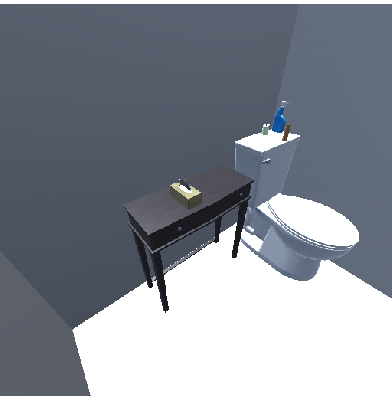
\includegraphics[width=\linewidth]{figures/epact_fig_handoff.pdf}
\end{minipage}\hfill
\begin{minipage}{0.6\linewidth}
\small
\textbf{Question:} Is there a TissueBox on the SideTable in the Bathroom?\\[3pt]
\textbf{Fresh-view QA:} yes (correct).\\[3pt]
\textbf{Interactive policy:} \texttt{LookAt(query\_location, center)} twelve times, then the decision limit. Every policy input image matches the fresh handoff image.
\end{minipage}
\caption{\textbf{Readable evidence, failed completion.} A frozen 8B handoff case. QA and policy calls see the same image with different prompts and output spaces; the QA answer is not passed to the policy.}
\label{fig:handoff}
\end{figure}

\begin{table}[htbp]
\centering
\caption{Task families and pair counts. Each pair contains two episodes with opposite answers.}
\label{tab:families}
\begin{tabular}{llrr}
\toprule
Family & Condition & Training pairs & Development pairs \\
\midrule
C & Closed container & 7 & 10 \\
D & Distance or viewpoint & 14 & 10 \\
L & Low light & 10 & 10 \\
C+D & Container and distance & 6 & 10 \\
L+D & Low light and distance & 11 & 10 \\
D+door & Distance with a closed doorway & 5 & 3 \\
N & Initially readable comparison & 12 & 10 \\
STATE$|$D & Object state under distance & 22 & 9 \\
\midrule
Total & & 87 & 72 \\
\bottomrule
\end{tabular}
\end{table}

\begin{figure}[htbp]
\centering
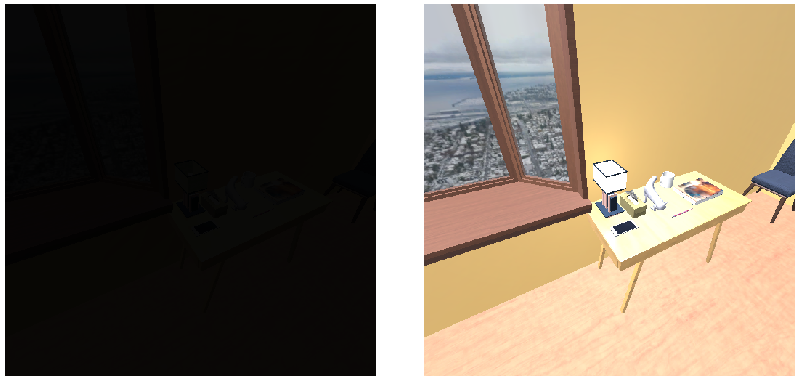
\includegraphics[width=0.62\linewidth]{figures/epact_fig_light.pdf}
\caption{\textbf{The lighting intervention.} The same camera view before and after a successful \texttt{Toggle} in a fine-tuned policy's rollout; the queried bed is inspected later in this trajectory.}
\label{fig:light}
\end{figure}

\paragraph{Adaptation.} We adapt Qwen3-VL-8B-Instruct with rank-16 LoRA (scaling 32, no dropout) on the language attention query, key, value and output projections, keeping the base model and vision encoder frozen. Training uses BF16, AdamW with learning rate $10^{-4}$, batch size one with gradient accumulation eight, gradient clipping at one and one epoch (91 updates for the full set). Each of three seeds starts from the base model. \Cref{tab:families_sft} gives the full trajectory-SFT results by family.

\begin{table}[htbp]
\centering
\caption{Full trajectory SFT by family (correct pairs per seed).}
\label{tab:families_sft}
\begin{tabular}{lrrrr}
\toprule
Family & Seed 1 & Seed 2 & Seed 3 & Pairs \\
\midrule
C & 3 & 3 & 4 & 10 \\
D & 6 & 6 & 3 & 10 \\
L & 6 & 7 & 6 & 10 \\
C+D & 3 & 3 & 3 & 10 \\
L+D & 8 & 10 & 6 & 10 \\
D+door & 1 & 0 & 0 & 3 \\
N & 6 & 7 & 6 & 10 \\
STATE$|$D & 6 & 6 & 6 & 9 \\
\midrule
Total & 39 & 42 & 34 & 72 \\
\bottomrule
\end{tabular}
\end{table}

\section{RL objective and execution}
\label{app:rl}
With $T$ the number of retained response tokens, the objective is
\begin{align}
\mathcal{L} &= \frac{1}{T}\sum_{e,t}\Big[-A_e\log\pi_\theta(y_{e,t}\mid h_{e,t}) + \beta\big(\exp(d_{e,t}) - d_{e,t} - 1\big)\Big],\\
d_{e,t} &= \log\pi_{A0}(y_{e,t}\mid h_{e,t}) - \log\pi_\theta(y_{e,t}\mid h_{e,t}),
\end{align}
with $\beta = 0.04$. Groups with uniform outcomes have zero advantage and are skipped, including their KL contribution. The objective has no clipped probability-ratio term. Each batch receives one AdamW update (learning rate $10^{-5}$, zero weight decay, gradient clipping at 1.0) with persistent optimizer state. Training samples at temperature 1; final evaluation is greedy with a 14-decision cap. The final checkpoint is used, and monitor probes were logged rather than used for checkpoint selection. A2 repeats the original 510 source SFT rows with a fresh shuffle, matching A1's update count; update matching does not imply matched rollout or token exposure. P executes 20 updates and 800 episodes.

Execution fell below the original 2,400-group design (25\%) and the first 1,440-group implementation plan (41.7\%). A throughput amendment first reduced the schedule to 36 updates of five groups; a later amendment restored 120 updates before target evaluation. One update before a logging fix is unobserved. Segment B has weaker inspection evidence: correct pairs sometimes occur with little target opening. We therefore keep the segment split rather than treating its validation as equivalent to segment A.

\section{Pre-specified criteria}
The internal plans fixed these thresholds before the corresponding runs: A1 must exceed A2 by four pairs (observed: three); the two SFT replication seeds must average 15 pairs on the reason-first test (observed: 12); secondary egg training must reach a mean of 9 of 12 with a minimum of 8 under retention constraints (neither scheme passes). Step-0 probes sample at temperature 1; final target evaluations are greedy. These are internal criteria, not public registrations.

\section{Reproducibility}
\label{app:repro}
The companion materials, included as ancillary files with this preprint, provide the benchmark CLI for the action-only and reason-first protocols with saved evaluation recipes, compact scoring records, two witness renders and their figure inputs; a CPU replay recomputes 119 reported values from 1,644 scoring records. Exact frozen task definitions for the 72 development and 55 target pairs are included, with original IDs, scene selections, modifications, starts and oracle plans; the target set reuses 32 development pairs. The 352 original start views are preserved in two separately checksummed companion archives. The compact ancillary bundle includes their manifest and restoration checks, but not the image archives; these are separate from the inputs needed for the CPU score replay. The house-input hash and simulator build are pinned, while upstream scene assets remain external. The full original training/episode attachment and the RL training orchestrator remain private. The generator is included, but regenerated scenes have not been verified as byte-identical. Code is released under the MIT license; third-party redistribution permissions remain separate. The public materials support inspection of the method, recomputation of saved scores and figure regeneration. They do not reproduce historical training or establish identical rerendering; relocated model and simulator execution has not yet been rerun. \Cref{fig:egg} embeds the two recorded witness PNGs at native resolution with unmodified pixel values; the crops are taken at recorded pixel coordinates and enlarged only by display scaling, each image is identified by its SHA-256 hash in the project records, and the answers shown are the recorded model outputs with and without the class note. The egg and non-egg strata, opening counts and light-call episode counts in \cref{tab:target} are computed from the recorded episodes of each policy (110 per policy); a light-call episode contains at least one issued \texttt{GoTo} or \texttt{Toggle} call whose target is \texttt{room\_light}.


\end{document}
